\documentclass{article}

\usepackage{graphicx}
\usepackage{tikz}
\usepackage{tikzsymbols}
\usetikzlibrary{calc,patterns,shapes.geometric}
\pagestyle{empty}
\usepackage[margin=0pt]{geometry}
\geometry{papersize={14in,12in}}

\def\centerarc[#1](#2)(#3:#4:#5){\draw[#1] ($(#2)+({#5*cos(#3)},{#5*sin(#3)})$) arc (#3:#4:#5);}

\begin{document}
	\begin{figure}
		\centering
		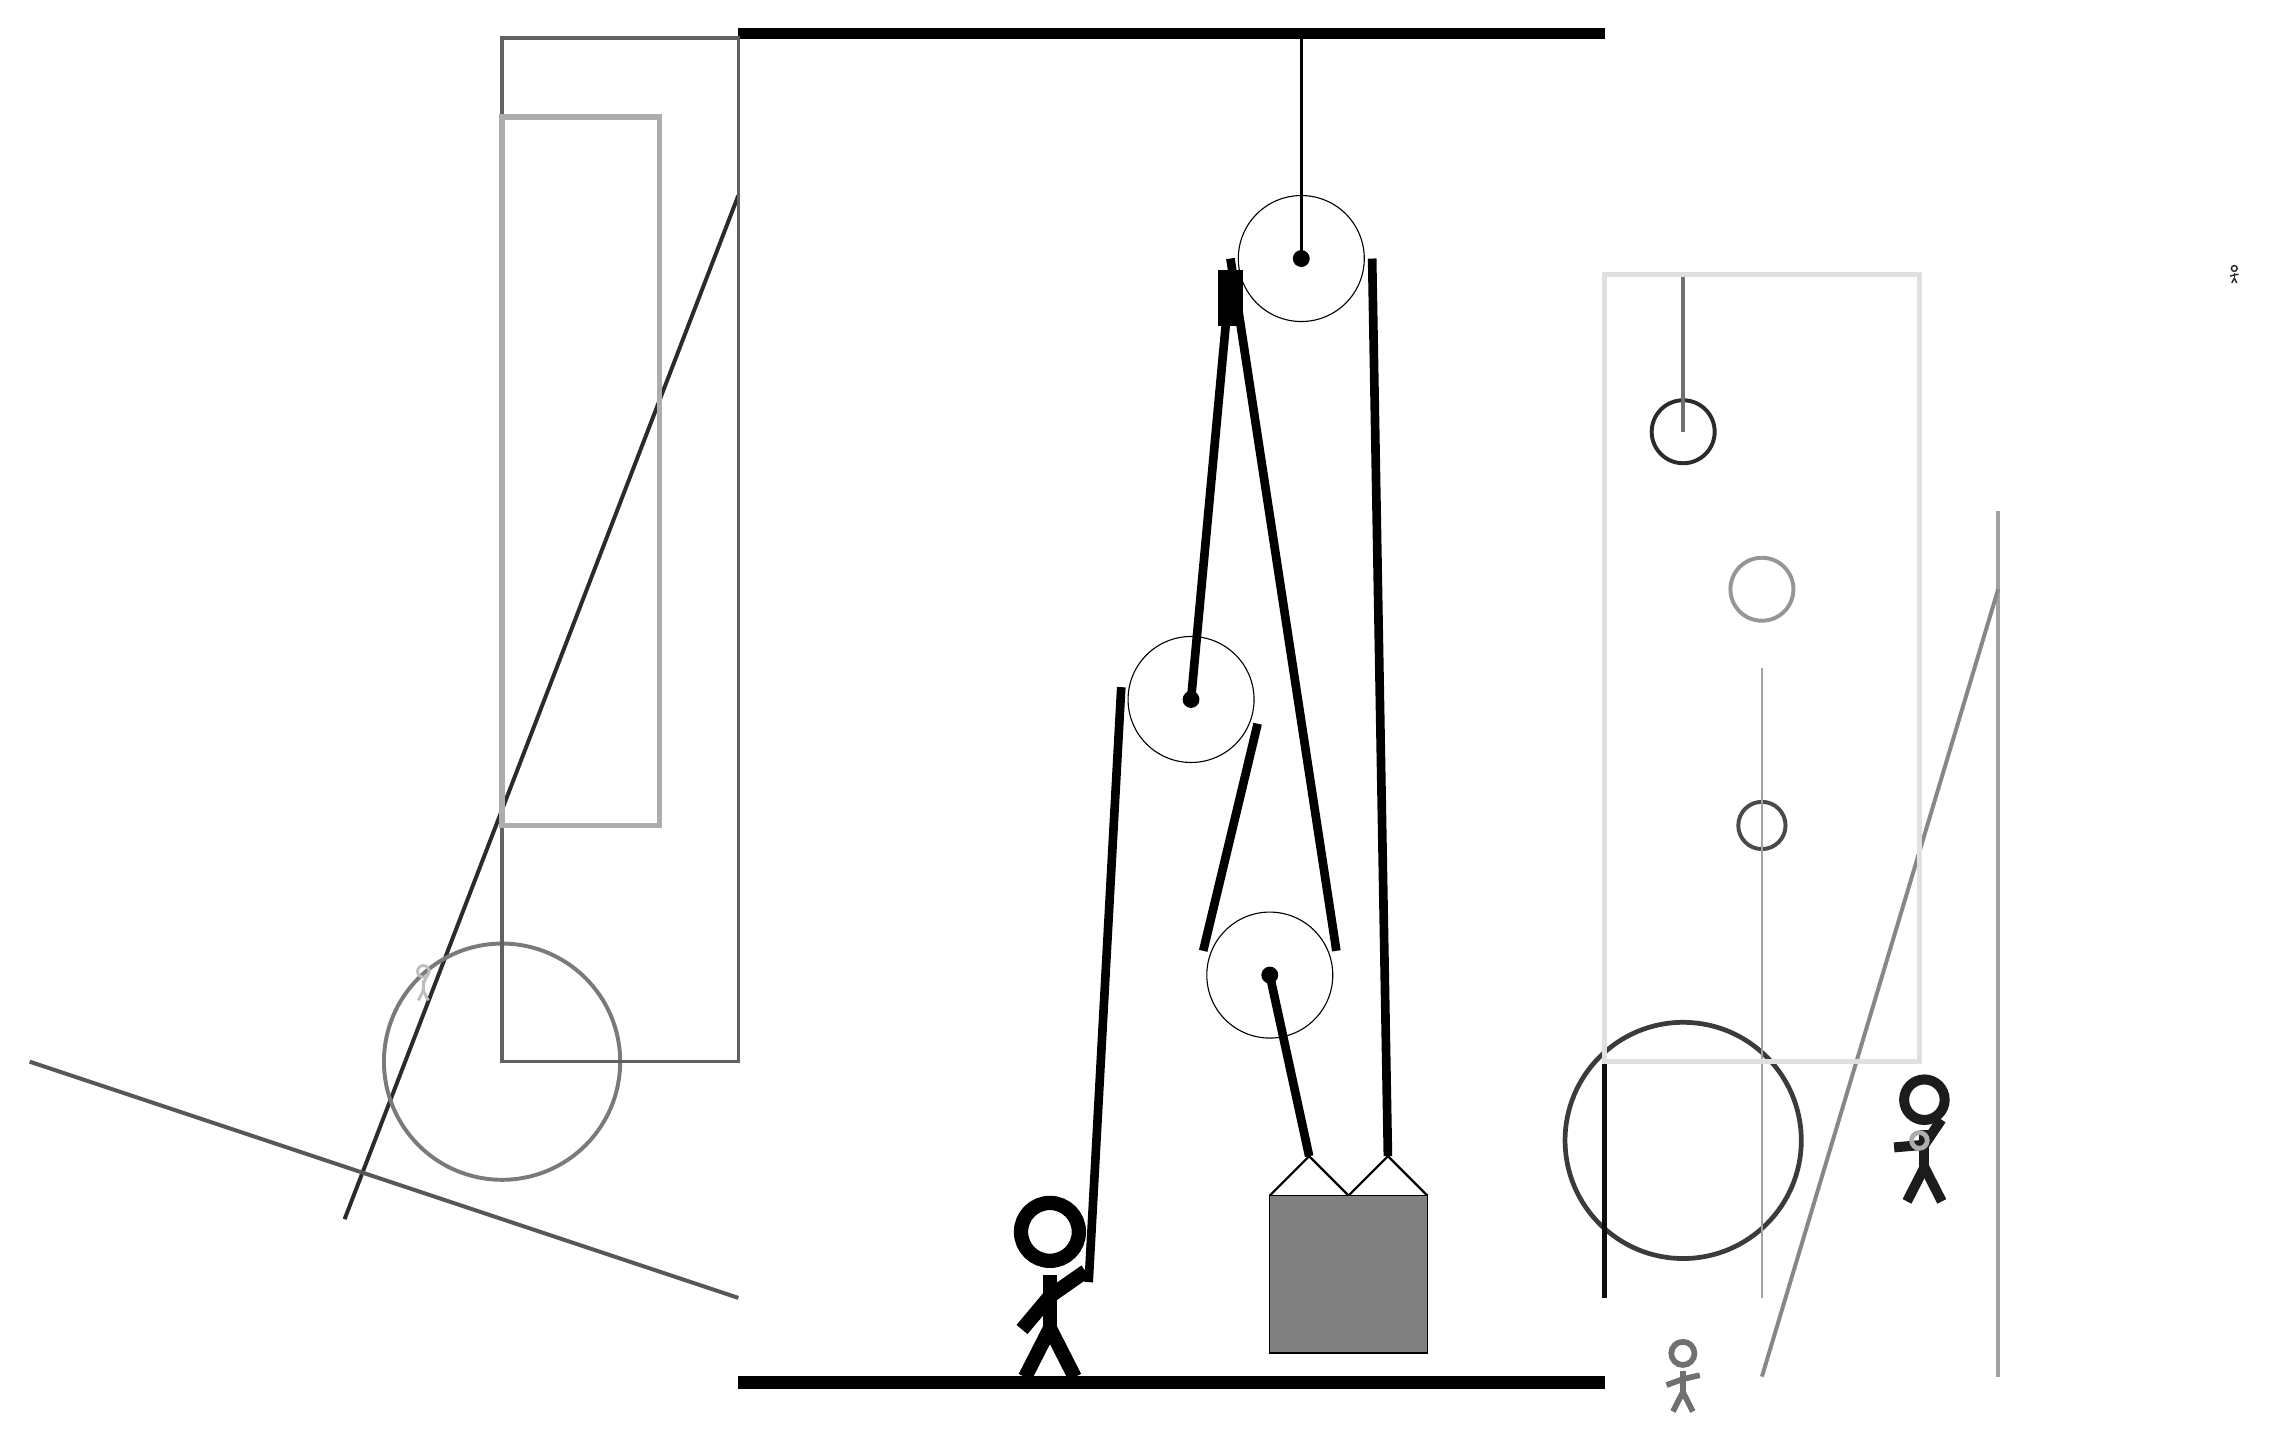
\begin{tikzpicture}
			%%%%% START %%%%%
			
			\draw[fill=black] (-6, 14) rectangle (5, 14.125);
			
			\draw (-0.25, 5.6) circle (0.8);
			\draw[fill=black] (-0.25, 5.6) circle (0.1);
			
			\draw (0.75, 2.1) circle (0.8);
			\draw[fill=black] (0.75, 2.1) circle (0.1);
			
			\draw (1.15, 11.2) circle (0.8);
			\draw[fill=black] (1.15, 11.2) circle (0.1);
			\draw[very thick] (1.15, 11.2) -- (1.15, 14);
			
			\draw[line width=0.5mm, color=black!83](-6, 12) -- (-11, -1);
			
			\node[line width=0.7mm, color=black!85] at (13, 11) {\Strichmaxerl[1][16][8]};
			\draw [line width=0.5mm, color=black!41](7, 7) circle (0.4);
			\draw [line width=0.5mm, color=black!52](-9, 1) circle (1.5);
			\draw [line width=0.6mm, color=black!77](6, 0) circle (1.5);
			\draw[line width=0.4mm, color=black!62] (-6, 1) rectangle (-9, 14);
			\draw[line width=0.7mm, color=black!32] (-7, 4) rectangle (-9, 13);
			\node[line width=0.3mm, color=black!56] at (6, -3) {\Strichmaxerl[4][20][13]};
			\draw [line width=0.5mm, color=black!83](6, 9) circle (0.4);
			\node[line width=0.7mm, color=black!89] at (9, 0) {\Strichmaxerl[7][5][56]};
			\draw[line width=0.5mm, color=black!56](6, 11) -- (6, 9);
			\draw[line width=0.5mm, color=black!37](10, -3) -- (10, 8);
			\draw [line width=0.6mm, color=black!32](9, 0) circle (0.1);
			
			\draw [line width=0.5mm, color=black!71](7, 4) circle (0.3);
			\draw[line width=0.5mm, color=black!47](7, -3) -- (10, 7);
			\node[line width=0.6mm, color=black!26] at (-10, 2) {\Strichmaxerl[2][88][67]};
			
			\draw[line width=0.2mm, color=black!36] (7, -2) rectangle (7, 6);
			\draw[line width=0.5mm, color=black!66](-6, -2) -- (-15, 1);
			\draw[line width=0.7mm, color=black!95] (5, -2) rectangle (5, 7);
			\draw[line width=0.7mm, color=black!12] (5, 11) rectangle (9, 1);
			
			\draw[thick]  (0.75, -0.7) -- (1.25, -0.2) -- (1.75, -0.7) -- (2.25, -0.2) -- (2.75, -0.7);
			\draw[fill=black!50] (0.75, -0.7) rectangle (2.75, -2.7);
			
			\draw[line width=1.1mm] (-0.25, 5.6) -- (0.25, 11.0);
			\draw[line width=1.1mm, fill=black](0.15, 10.4) rectangle (0.35, 11.0);
			\draw[line width=1.1mm] (-1.55, -1.8) -- (-1.1363, 5.7562);
			\centerarc[line width=1.1mm](-0.25, 5.6)(-20:170:0.9);
			\draw[line width=1.1mm] (0.5957, 5.2922) -- (-0.0957, 2.4078);
			\centerarc[line width=1.1mm](0.75, 2.1)(160:380:0.9);
			\draw[line width=1.1mm] (1.5957, 2.4078) -- (0.25, 11.2);
			\draw[line width=1.1mm](0.75, 2.1) -- (1.25, -0.2);
			\centerarc[line width=1.1mm](1.15, 11.2)(0:180:0.9);
			\draw[line width=1.1mm] (2.05, 11.2) -- (2.25, -0.2);
			
			\node at (-2, -1.9) {\Strichmaxerl[10][50][35]};
			
			\draw[fill=black] (-6, -3) rectangle (5, -3.15);
			
			%%%%% END %%%%%
		\end{tikzpicture}
	\end{figure}	
\end{document}